\chapter{INFRAESTRUTURA EM NUVEM E DEVOPS}

Durante o desenvolvimento, a solução foi executada localmente, com o SQL Server em um contêiner Docker. Este capítulo apresenta a proposta de implantação em produção, que ainda não foi executada. A computação em nuvem foi escolhida por oferecer recursos sob demanda, elasticidade e cobrança proporcional ao uso \cite{mell2011}, características adequadas a uma distribuidora que não mantém equipe de infraestrutura.

\section{Arquitetura em nuvem e serviços utilizados}

A proposta usa o modelo de Plataforma como Serviço (PaaS) no Microsoft Azure, escolhido pela integração nativa com .NET e SQL Server. A Figura~\ref{fig:nuvem} mostra o caminho do código até a produção e os serviços envolvidos, detalhados na Tabela~\ref{tab:servicos}.

\begin{figure}[htbp]
\centering
\caption{Arquitetura em nuvem e esteira de entrega proposta}
\label{fig:nuvem}
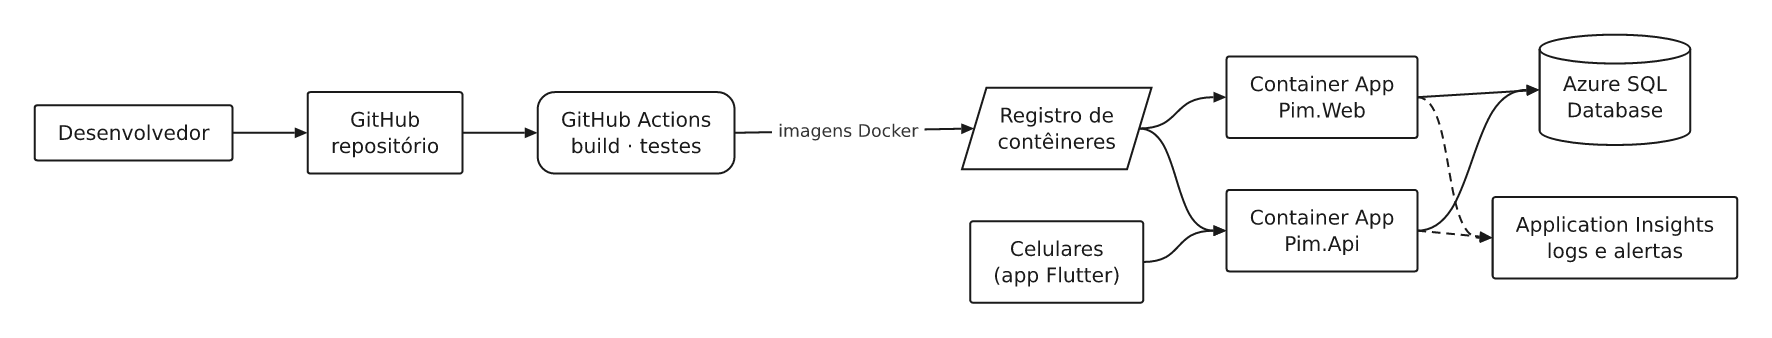
\includegraphics{figuras/nuvem.png}
\fonte{Elaborado pelo autor (2026)}
\end{figure}

\begin{table}[htbp]
\centering
\caption{Serviços de nuvem propostos}
\label{tab:servicos}
\footnotesize
\begin{tabular}{|p{4cm}|p{10.4cm}|}
\hline
\textbf{Serviço} & \textbf{Uso na solução} \\ \hline
Azure Container Apps & Executa os contêineres do \texttt{Pim.Web} e do \texttt{Pim.Api}, com HTTPS e escala automática \\ \hline
Azure Container Registry & Guarda as imagens Docker geradas pela integração contínua \\ \hline
Azure SQL Database & Banco gerenciado, com \textit{backup} automático e restauração para um ponto no tempo \\ \hline
Azure Key Vault & Guarda a string de conexão e a chave de assinatura do JWT fora do código \\ \hline
Application Insights & Coleta logs, tempos de resposta, falhas e dispara alertas \\ \hline
GitHub Actions & Executa a esteira de integração e entrega contínuas \\ \hline
\end{tabular}
\fonte{Elaborado pelo autor (2026)}
\end{table}

\section{Contêineres e pipeline CI/CD}

Cada aplicação é empacotada em uma imagem Docker, o que garante que o mesmo artefato testado seja o executado em produção. O código a seguir mostra o \textit{Dockerfile} proposto para a API, em dois estágios: o primeiro compila com o SDK e o segundo contém apenas o \textit{runtime}, resultando em uma imagem menor e com menos superfície de ataque.

\begin{codeblock}[Dockerfile proposto para a API]{bash}
FROM mcr.microsoft.com/dotnet/sdk:10.0 AS build
WORKDIR /src
COPY . .
RUN dotnet publish Pim.Api -c Release -o /app

FROM mcr.microsoft.com/dotnet/aspnet:10.0
WORKDIR /app
COPY --from=build /app .
ENTRYPOINT ["dotnet", "Pim.Api.dll"]
\end{codeblock}

A esteira segue as práticas de integração e entrega contínuas \cite{humble2014}. A cada \textit{push}, o GitHub Actions compila a solução, executa o analisador do Flutter e os testes de unidade e, com um SQL Server em contêiner efêmero, os testes de ponta a ponta. Se tudo passar na ramificação principal, as imagens são publicadas no registro e implantadas primeiro em um ambiente de homologação; a promoção para produção é feita após aprovação. Antes da implantação, uma etapa própria da esteira aplica as \textit{migrations} pendentes ao banco; a aplicação automática na inicialização fica restrita ao ambiente de desenvolvimento. O aplicativo Android é gerado na mesma esteira e distribuído pela loja em modo de teste fechado.

\section{Monitoramento, escalabilidade e segurança}

O monitoramento usa o Application Insights para acompanhar disponibilidade, tempo de resposta das rotas de bipagem e taxa de erros, com alertas quando o tempo médio ultrapassar um segundo ou quando houver falhas seguidas, seguindo a ideia de \textit{feedback} rápido da cultura DevOps \cite{kim2018}. A escalabilidade é horizontal: a API não guarda estado em memória, já que o login é carregado no próprio token, e por isso o Container Apps pode criar novas instâncias nos horários de pico de carregamento e reduzi-las fora do expediente. O banco pode ter sua capacidade ajustada sem alteração no código.

Na segurança, todo o tráfego usa HTTPS; segredos ficam no Key Vault, e não no repositório; o banco aceita conexões apenas da rede da aplicação; e as imagens são verificadas quanto a vulnerabilidades conhecidas antes da publicação. A chave de desenvolvimento do JWT, presente no arquivo de configuração local, deve ser substituída por uma chave gerada e guardada no Key Vault.
